\chapter{Methods}\label{ch:methods}

\begin{chapterabstract}
    In the following chapter, we outline the methods of work used to assess the Gaia-X initiative, the reference framework implementation by GXFS and answer the research questions stated in the introductory Chapter~\ref{ch:introduction}.
    The main method of work is implementation of a Gaia-X-compliant data exchange module, serving as a proof of concept.
    Based on this, we note the Gaia-X related technical challenges.
    Additionally, we take a closer look on the architecture of Gaia-X and at the project in which we implement the data exchange module.
    Lastly, we present a selection of risks and metrics identified in the previous Chapter~\ref{ch:related-work} --- Related Work.
\end{chapterabstract}

\section{About Carecentive}\label{sec:about-carecentive}

Carecentive~\cite{carecentive} is a backend software framework used for supporting health studies and trials.
The framework offers features that are typically required in medical trials, notably the following:
\begin{itemize}
    \item User management (registration, login, password management)
    \item Questionnaire storage \& submission
    \item Activity scheduling (e.g., periodical questionnaire submission)
    \item File upload (e.g., images of medical records)
    \item Wearable devices integration (Withings API, Fitbit API)
    \item User activity analytics
    \item Permission management (Roles such as patients, relatives, physicians, nurses, study managers)
\end{itemize}

\subsection{Tech Stack}\label{subsec:tech-stack}

From the developmental standpoint, the framework is divided into two packages, \textit{carecentive-framework}\footnote{https://github.com/carecentive/carecentive-framework} which mainly sets up the application, registers and exposes the API on the outside.
The API requests are then handed over to the main package \textit{carecentive-code}\footnote{https://github.com/carecentive/carecentive-core}, which does the heavy lifting of handling user requests based on its business logic.

The Carecentive is written in the \textit{JavaScript} programming language and is running in the \textit{Node.js} engine.
It is built on top of the \textit{Express} web framework, enabling the RESTful API interface, stores data in the relational MySQL DBMS (Database Management Systems).
The database tables are versioned via database migrations enabled by the\textit{Knex.js} library, and relational data is mapped onto objects (models) using the \textit{Objection.js} library.

%TODO: add references to the libraries
In order to simplify setting up the project on different machines and improve stability, we also used the Docker platform, which ensures installation of all dependencies and runs the app in an isolated environment, reducing the differences in various operating systems.
%TODO: should I explain this more?

\subsection{Use Cases}\label{subsec:use-cases}

The framework was developed in the FAU (Friedrich-Alexander-Universität) MaD (Machine Learning and Data Analytics) Lab, under which I'm working on this thesis.
Currently, a smartphone app is used as a frontend for the Carecentive backend counterpart in a running study investigating the health of patients receiving care at the palliative care unit in the \textit{Uniklinikum Erlangen} (University Hospital Erlangen).
Thanks to the extensibility of the Carecentive framework, it was also utilized in the works of other students doing their thesis under the FAU MaD Lab (e.g., Smartphone-based Urinalysis).

%TODO: add screenshots of the app

In order to assess the functionality of the Gaia-X ecosystem, a partial goal of this thesis is to implement a Gaia-X-compliant module for the exchange of the data stored in the Carecentive app.
During the implementation of the exchange module, serving as a proof of concept, we note of any technical or other issues with the Gaia-X specifications and with the GXFS software.
After the implementation is finished, we run a set of predefined data exchange scenarios to verify the correct functionality of our implementation and mainly whether the Gaia-X and GXFS software is ready for a real-world usage.
This is done with in the specific use-case of the palliative care trial.

\section{Gaia-X Concepts}\label{sec:gaia-x-concepts}

\subsection{Credentials}\label{subsec:credentials}

%TODO: replace Self-Desctiptions with Gaia-X Credentials
Gaia-X Credentials, formerly known as Gaia-X Self-Descriptions, are the main conceptual building blocks of the Gaia-X ecosystem~\cite{gaiax_architecture_document}.
They formalize all the claims and descriptions made by all parties participating in the ecosystem.
They are based on the formal \textit{Verifiable Credentials Data Model}~\cite{verifiable_credentials} specification issued by the \textit{World Wide Web Consortium} (W3C) and on the concept of Linked Data (LD).

Verifiable Credentials are inspired by physical credentials like government-issued passports, driving licenses and university diplomas.
They contain information about some statements the credential holder is trying to prove (citizenship, achieved education, etc.) and are secured by some protective element from the issuer, proving the veracity of the document, which the verifier can verify.
Their software counterpart (VCs) work in a similar way.
They contain data with relevance to the holder, which is structured based on well-defined templates called schemas or vocabularies, which describe which claims can be made in the document.

The claim consists of a subject (credential holder), property and a value, for example, Pat being an alumni of ``Example University''~\ref{fig:verifiable-credential-claim}.
These claims are then packed into the credential body along with metadata such as the issuer, issuance date or the expiration date.
Although other formats are permitted, the base format VCs are encoded in is the JSON (JavaScript Object Notation) format or more specifically the extension for Linked Data --- JSON-LD, this ensures the data is machine-readable and can be interlinked between each other.
The issuer then signs the credential using digital signature proving, which is inserted into the VC's proof section.
This provides a machine-readable cryptographical proof, which secures the credential and can be used by the verifier to verify holder's claims.

\begin{figure}
    \centering
    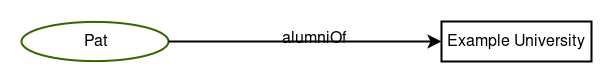
\includegraphics[width=\textwidth]{figures/verifiable-credential-claim-example.png}
    \caption{An example claim expressing Pat being an alumni of ``Example University''~\cite{verifiable_credentials}}\label{fig:verifiable-credential-claim}
\end{figure}
%TODO: fix svg figures
\begin{figure}
    \centering
    
\includegraphics[width=\textwidth]{figures/verifiable-credentials.png}
    \caption{Verifiable Credential roles and information flow~\cite{verifiable_credentials}}\label{fig:verifiable-credentials}
\end{figure}

Gaia-X utilizes VCs for almost all of the objects in the ecosystem from the \texttt{Participant}, serving as a description of a natural person or a legal entity, to the \texttt{ServiceOffering} and \texttt{Resource} credentials, specifying the offered services or data.
Gaia-X provides the so-called \textit{Gaia-X Trust Framework} via which the syntactic correctness, schema validity, cryptographic signature validation, attribute value consistency and attribute value verification is enforced~\cite{gaiax_architecture_document}.
This is done to ensure compliance with the minimal requirements defined by Gaia-X specifications is met.
However, thanks to the possible extensibility of the VC schemas, each federation can impose new rules for the credentials which federation Participants have to obey.

\begin{figure}
\centering
\begin{minted}[bgcolor=LightGray,breaklines]{json}
{
  "@context": [
    "https://www.w3.org/2018/credentials/v1",
    "https://w3id.org/security/suites/jws-2020/v1",
    "https://registry.lab.gaia-x.eu/development/api/trusted-shape-registry/v1/shapes/jsonld/trustframework#"
  ],
  "type": [
    "VerifiableCredential"
  ],
  "id": "https://gaia-x-dev.simerda.dev/gaia-x/john-doe/participant.json",
  "issuer": "did:web:gaia-x-dev.simerda.dev:gaia-x:john-doe",
  "issuanceDate": "2024-08-13T17:50:27.483+00:00",
  "credentialSubject": {
    "id": "https://gaia-x-dev.simerda.dev/gaia-x/john-doe/participant.json#cs",
    "type": "gx:LegalParticipant",
    "gx:legalName": "Example Enterprise",
    "gx:legalRegistrationNumber": {
      "id": "https://gaia-x-dev.simerda.dev/gaia-x/john-doe/legal-registration-number.json#cs"
    },
    "gx:headquarterAddress": {
      "gx:countrySubdivisionCode": "CZ-52"
    },
    "gx:legalAddress": {
      "gx:countrySubdivisionCode": "CZ-52"
    }
  },
  "proof": {
    "created": "2024-08-13T17:50:28.392+00:00",
    "type": "JsonWebSignature2020",
    "proofPurpose": "assertionMethod",
    "verificationMethod": "did:web:gaia-x-dev.simerda.dev:gaia-x:john-doe#JWK2020-RSA",
    "jws": "eyJhbGciOiJQUzI1NiIsImI2NCI6ZmFsc2UsImNyaXQiOlsiYjY0Il19..cPShjGoSpCKGfjU6pvjQnGeXCiN36smCdSpkPwp6Ruf24bSzvKQ2Slg9mve84-ZbEaVJVhtn6q1p833xaCAI9m0h3EUnzctukottOGrdWD5pJG2EHwkDYYY_SrfOT_Y7uIYaSf46_2FPAzvHxGoTRGPkvR-6cPmV_RW6Js6iagqmeOY1zjV89q4_2HibNnGWRLIAlWs1yrwk-3w4JEQWgQcilCa3xy_9i7L3mWyVE_4JC0HvXGVvanViIbr04xHdf--AkPlgO-eBItDogjL7pcUf0R7ORgB_ho7lP6OfbKht8Ru5PXNQjgfFJ2TO7zw9sJmaCRCqenCjn-QpfniMuA"
  }
}
\end{minted}
\caption{Example of a Gaia-X Participant Credential}\label{fig:gaia_x_credential_example}
\end{figure}

\subsection{Decentralized Identifiers}\label{subsec:decentralized-identifiers}

When creating a Verifiable Credential, it is necessary to be able to unambiguously identify the issuer, hence the W3C stipulates that the value of the \texttt{issuer} property must be a URL (Uniform Resource Locator) or object containing property \texttt{id} with URL as the value~\cite{verifiable_credentials}.
Gaia-X further restricts this rule, requiring the \texttt{issuer} property to contain a Decentralized Identifier (DID)~\cite{did}. %TODO: verify
DIDs are designed in a way to be used without the need to use centralized registries, which fits nicely into the ideology of Gaia-X.
While a third party may be needed to enable the discovery of information related to a DID, the design of enables the controller of a DID to prove its control over the Decentralized Identifier without requiring a permission from any other party.

The Figure~\ref{fig:did_structure} depicts the general structure of a Decentralized Identifier.
Gaia-X specifically uses the DID \texttt{web} method~\cite{didweb}, which allows holder to publish a DID document on a public webserver accessible using the HTTPS protocol.
For example, the DID \texttt{did:web:gaia-x-dev.simerda.dev:gaia-x:john-doe} gets resolved to the URL \url{https://gaia-x-dev.simerda.dev/gaia-x/john-doe/did.json}.
The resolved URL then host a document containing the ID itself and mainly the verification method and algorithms used with this DID.
The example document corresponding to the example DID can be seen in Figure~\ref{fig:did_document}; it specifies the X.509 certificate used and algorithm used for signing (RS256).
In relation to VCs and Gaia-X Credentials, the verifier of the credential can resolve the DID document and use the information provided to verify the signature included in the credential.

\begin{figure}
    \centering
    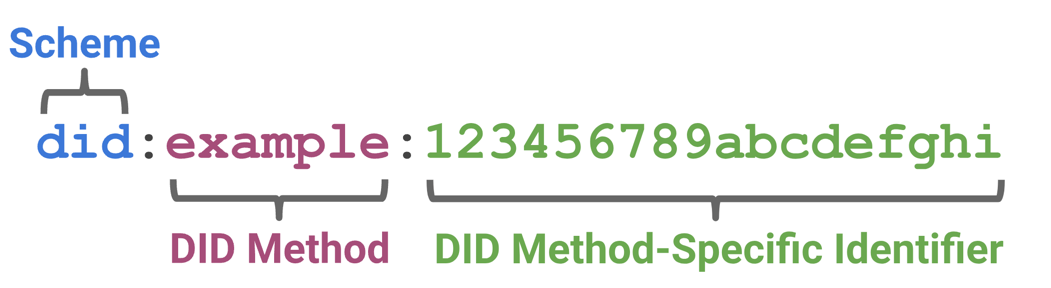
\includegraphics[width=0.7\textwidth]{figures/parts-of-a-did.png}
    \caption{Structure of a Decentralized Identifier~\cite{did}}\label{fig:did_structure}
\end{figure}

\begin{figure}
\centering
\begin{minted}[bgcolor=LightGray,breaklines]{json}
{
  "@context": [
    "https://www.w3.org/ns/did/v1",
    "https://w3id.org/security/suites/jws-2020/v1"
  ],
  "id": "did:web:gaia-x-dev.simerda.dev:gaia-x:john-doe",
  "verificationMethod": [
    {
      "id": "did:web:gaia-x-dev.simerda.dev:gaia-x:john-doe#JWK2020-RSA",
      "type": "JsonWebKey2020",
      "controller": "did:web:gaia-x-dev.simerda.dev:gaia-x:john-doe",
      "publicKeyJwk": {
        "kty": "RSA",
        "n": "1BQuEryN-A0p-TI8HOtN5xB8rwbyUre4e0fhUiPECFvd58xX_gsiMFqrsDb3ZcrnaE-0o4StXy5A0GFBouuwGX1UlZQ1V9PiPXbd05vAbv4T7xGeAuzhDbgZviiJb-SsLFAZQc6UDC5eeM1x7_KWgRCB82Nc9BGfCxLz3U6dyzrUZq8VKn9S3mkKLLuslewa00X8TCHEAVQFEktVV9F617GXEknrEZhKoZfPeuiweMj4FxuamBRQPaZlCWQduiDnVkmNu4pr7C7HJQkBxxH-D32IhxGrSg1mQtaSO-wbYgqVMoDyWFmdUGoiQmocXWKwRBC0zuxvxgninAB7wTywbQ",
        "e": "AQAB",
        "alg": "RS256",
        "x5u": "https://gaia-x-dev.simerda.dev/gaia-x/john-doe/cert.pem"
      }
    }
  ],
  "assertionMethod": [
    "did:web:gaia-x-dev.simerda.dev:gaia-x:john-doe#JWK2020-RSA"
  ]
}
\end{minted}
\caption{Example of a DID document}\label{fig:did_document}
\end{figure}

\subsection{Trust Anchors}\label{subsec:trust-anchors}

Trust Anchors are entities that underpin the claims by Participants and are endorsed by Gaia-X~\cite{gaiax_trust_framework}.
They facilitate the processing of claims made by Participants and shall do so via fair and transparent procedures and thus affirm the trust in otherwise mere self-declared statements.
Trust Anchors may underpin any aspect of the Participant's operation; however, Gaia-X will only be interested in aspects relating to criteria relevant stemming from the issued specifications.

In reality, the abstract term ``Trust Anchors'' primarily refers to the Trust Service Providers (TSPs) or Certification Authorities (CAs) from which a Participant is permitted to obtain digital certificates.
Notable exception is for the Credential \texttt(legalRegistrationNumber), where the Gaia-X Association nominated itself as a valid Trust Anchor for the purpose of validating legal person's registration numbers via the notary service.
These certificates are necessary for signing Gaia-X Credentials to ensure trust and compliance with Gaia-X standards.
The exact permissible Trust Anchors are defined in Table~\ref{tab:trust_anchors}.

\begin{figure}
    \centering
    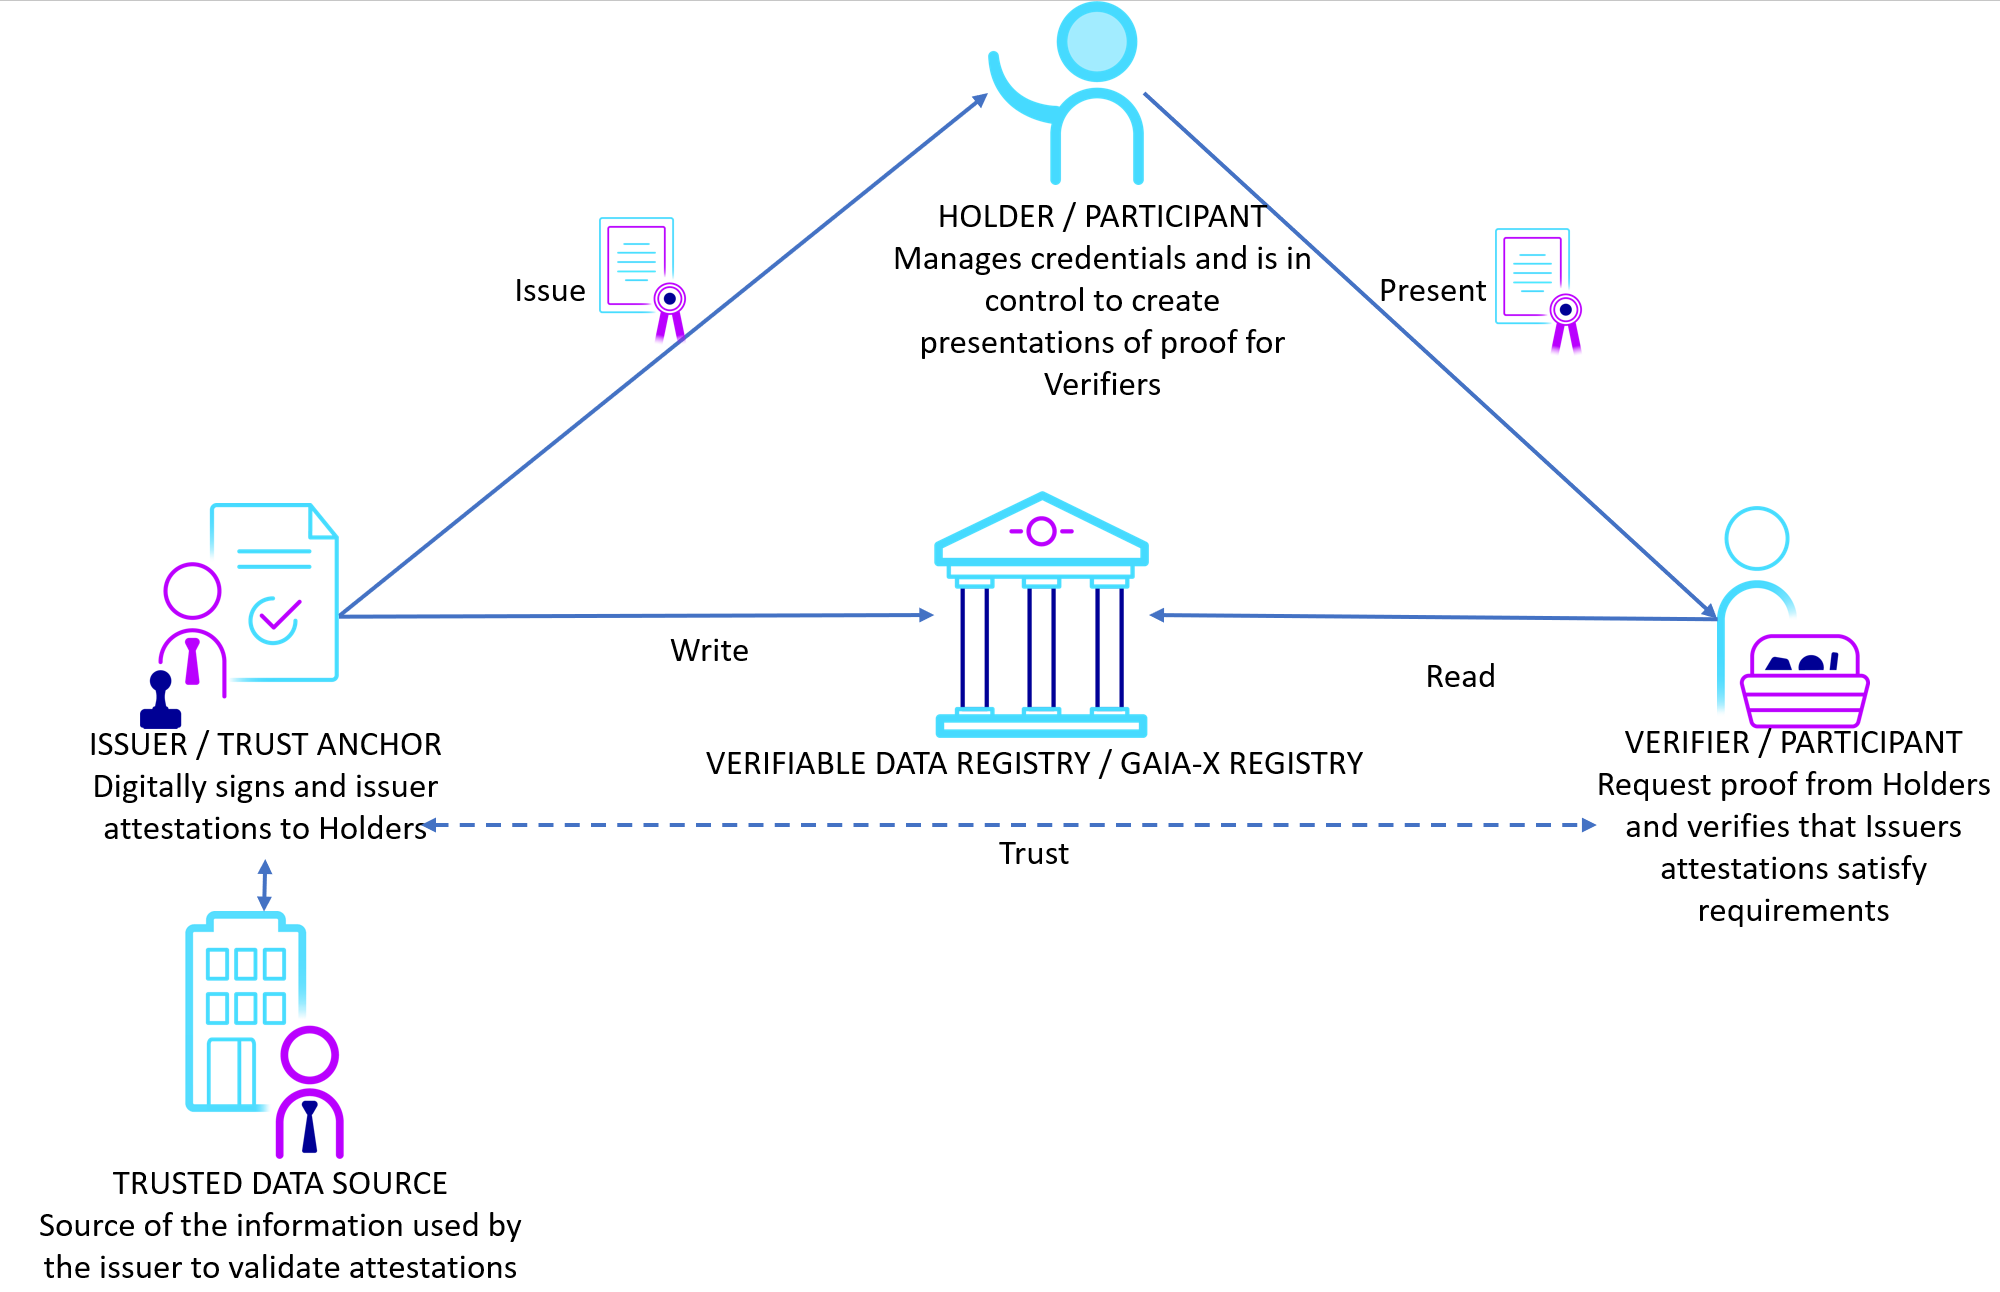
\includegraphics[width=\textwidth]{figures/vc_model.png}
    \caption{Interactions among different Participant roles in the Gaia-X Trust Framework~\cite{gaiax_trust_framework}}\label{fig:trust_framework_interactions}
\end{figure}

\begin{table}
    \centering
    {\renewcommand{\arraystretch}{1.7}
        \begin{tabular}{ |p{4cm}|p{11cm}| }
            \textbf{Name} & \textbf{Defined as}\\
            \hhline{--}
            State & The Trust Service Providers (TSP) must be a state validated identity issuers or EV SSL issuers.
            - For participant, if the legalAddress.country is in EEA, valid state identity issuers are eiDAS ones.
            - Gaia-X Association may also be a valid TSP for Gaia-X Association members.\\
            \hhline{--}
            eiDAS & Issuers of Qualified Certificate for Electronic Signature as defined in eIDAS Regulation (EU) No 910/2014
            (homepage: https://esignature.ec.europa.eu/efda/tl-browser/\#/screen/home)
            (machine: https://ec.europa.eu/tools/lotl/eu-lotl.xml)\\
            \hhline{--}
            EV SSL & Extended Validation (EV) Secure Sockets Layer (SSL) certificate issuers are considered to be temporarily valid Trust Service Providers.
            (homepage: https://wiki.mozilla.org/CA/Included\_Certificates)
            (machine: https://ccadb-public.secure.force.com/mozilla/IncludedCACertificateReportPEMCSV)\\
            \hhline{--}
            registrationNumberIssuer & During the pilot phase, the Gaia-X Association nominated itself as a valid Trust Anchor under https://notary.gaia-x.eu
        \end{tabular}
    }
    \caption{Trust Anchors~\cite{gaiax_trust_framework}}
    \label{tab:trust_anchors}
\end{table}

%TODO: policies

\subsection{Trust Framework Components}\label{subsec:trust-framework-components}

This section describes the software components which are operated by the Gaia-X Digital Clearing Houses (GXDCHs).
Gaia-X Digital Clearing House~\cite{gaiax} is a term describing a network of execution nodes, they operationalize the theoretical Gaia-X Framework by enforcing the set of rules defined in Gaia-X specifications and provide a Gaia-X compliance.
Along with \textit{Gaia-X Lab}\footnote{A team of developers working under the umbrella of the Gaia-X Association}, the services are operated by four other companies, making it a decentralized system.
The GXCHs consist of three mandatory services --- Gaia-X Compliance, Gaia-X Registry and Gaia-X Notary.

\subsubsection{Gaia-X Compliance}

The purpose of this service is to accept Gaia-X Credentials (wrapped in a Verifiable Presentation), check them against the defined schemas and verify the validity of the Credentials using syntactic, consistency and cryptographical checks~\cite{gaiax_trust_framework}.
If all the checks pass, the service returns a Gaia-X Credential with a Gaia-X signature, as a proof that the input provided has passed all the verifications, proving Participant's compliance.

\subsubsection{Gaia-X Registry}

The Registry is a backbone of the Gaia-X ecosystem governance, acting as a non-repudiable, immutable and permissionless database\cite{gaiax_trust_framework}.
The database stores the following information:
\begin{itemize}
    \item the list of the Trust Anchors – keyring.
    \item the result of the Trust Anchors validation processes.
    \item the potential revocation of Trust Anchors' identity.
    \item the vote and results of the Gaia-X Association roll call vote, similar to the rules of the plenary of the European Parliament.
    \item the shapes and schemas for the Gaia-X VCs.
    \item the URLs of Gaia-X Catalogue’s credentials.
    \item the text of the Terms and Conditions for Gaia-X Conformity.
\end{itemize}

\subsubsection{Gaia-X Notary}

At the moment, the Notary service serves the singular purpose of validating the Participant's legal registration number~\cite{gaiax_trust_framework}.
It checks that the Gaia-X credential contains at least one of the permissible legal entity identification number stated in the Gaia-X specifications and validates it using external services.
Upon successful validation, it issues a Gaia-X Credential attesting to these claims.

In the future, the notary shall also perform notarization of Data Product Usage Contracts. %TODO: cite data exchange specification

\section{Implementation}\label{sec:implementation}

\textcolor{red}{This will be probably a shorter section about my concrete implementation of the data exchange module in the context of Carecentive.}

\section{Evaluation}\label{sec:evaluation}

In order to evaluate the actual state of the Gaia-X ecosystem, the following tests will be performed with using our implementation of the Carecentive exchange module.

\begin{enumerate}
    \item Obtaining Gaia-X compliance
    \item Creating Gaia-X credentials for data products
    \item Performing data exchange with questionnaire data
    \item Performing data exchange with withings data
\end{enumerate}

The results of these tests are presented in the following chapter.
